%%
%% Copyright 2007, 2008, 2009 Elsevier Ltd
%%
%% This file is part of the 'Elsarticle Bundle'.
%% ---------------------------------------------
%%
%% It may be distributed under the conditions of the LaTeX Project Public
%% License, either version 1.2 of this license or (at your option) any
%% later version.  The latest version of this license is in
%%    http://www.latex-project.org/lppl.txt
%% and version 1.2 or later is part of all distributions of LaTeX
%% version 1999/12/01 or later.
%%
%% The list of all files belonging to the 'Elsarticle Bundle' is
%% given in the file `manifest.txt'.
%%

%% Template article for Elsevier's document class `elsarticle'
%% with numbered style bibliographic references
%% SP 2008/03/01
%%
%%
%%
%% $Id: elsarticle-template-num.tex 4 2009-10-24 08:22:58Z rishi $
%%
%%
%\documentclass[preprint,12pt,3p]{elsarticle}

%% Use the option review to obtain double line spacing
\documentclass[preprint,review,12pt]{elsarticle}

%% Use the options 1p,twocolumn; 3p; 3p,twocolumn; 5p; or 5p,twocolumn
%% for a journal layout:
%% \documentclass[final,1p,times]{elsarticle}
%% \documentclass[final,1p,times,twocolumn]{elsarticle}
%% \documentclass[final,3p,times]{elsarticle}
%% \documentclass[final,3p,times,twocolumn]{elsarticle}
%% \documentclass[final,5p,times]{elsarticle}
%% \documentclass[final,5p,times,twocolumn]{elsarticle}

%% if you use PostScript figures in your article
%% use the graphics package for simple commands
%% \usepackage{graphics}
%% or use the graphicx package for more complicated commands
%% \usepackage{graphicx}
%% or use the epsfig package if you prefer to use the old commands
%% \usepackage{epsfig}

%% The amssymb package provides various useful mathematical symbols
\usepackage{amssymb}
%% The amsthm package provides extended theorem environments
%% \usepackage{amsthm}

%% The lineno packages adds line numbers. Start line numbering with
%% \begin{linenumbers}, end it with \end{linenumbers}. Or switch it on
%% for the whole article with \linenumbers after \end{frontmatter}.
%% \usepackage{lineno}

%% natbib.sty is loaded by default. However, natbib options can be
%% provided with \biboptions{...} command. Following options are
%% valid:

%%   round  -  round parentheses are used (default)
%%   square -  square brackets are used   [option]
%%   curly  -  curly braces are used      {option}
%%   angle  -  angle brackets are used    <option>
%%   semicolon  -  multiple citations separated by semi-colon
%%   colon  - same as semicolon, an earlier confusion
%%   comma  -  separated by comma
%%   numbers-  selects numerical citations
%%   super  -  numerical citations as superscripts
%%   sort   -  sorts multiple citations according to order in ref. list
%%   sort&compress   -  like sort, but also compresses numerical citations
%%   compress - compresses without sorting
%%
%% \biboptions{comma,round}

% \biboptions{}

\usepackage{graphicx}
\usepackage[space]{grffile}
\usepackage{latexsym}
\usepackage{amsfonts,amsmath,amssymb}
\usepackage{url}
\usepackage[utf8]{inputenc}
\usepackage{fancyref}
\usepackage{hyperref}
\hypersetup{colorlinks=false,pdfborder={0 0 0},}



\journal{Elsevier Journal}

\begin{document}

\begin{frontmatter}

%% Title, authors and addresses

%% use the tnoteref command within \title for footnotes;
%% use the tnotetext command for the associated footnote;
%% use the fnref command within \author or \address for footnotes;
%% use the fntext command for the associated footnote;
%% use the corref command within \author for corresponding author footnotes;
%% use the cortext command for the associated footnote;
%% use the ead command for the email address,
%% and the form \ead[url] for the home page:
%%
%% \title{Title\tnoteref{label1}}
%% \tnotetext[label1]{}
%% \author{Name\corref{cor1}\fnref{label2}}
%% \ead{email address}
%% \ead[url]{home page}
%% \fntext[label2]{}
%% \cortext[cor1]{}
%% \address{Address\fnref{label3}}
%% \fntext[label3]{}

\title{No Title Found}


\author[first]{Marcus Oelze}
\address[first]{GFZ Potsdam}




\begin{abstract}
No Abstract Found

\end{abstract}




%\begin{keyword}
%% keywords here, in the form: keyword \sep keyword

%% MSC codes here, in the form: \MSC code \sep code
%% or \MSC[2008] code \sep code (2000 is the default)

%\end{keyword}

\end{frontmatter}

\bibliographystyle{elsarticle-num}


Die Langmuir-Isotherme ist das einfachste Sorptionsmodell, das physikalische Grundlagen besitzt. 
Es geht von folgenden Annahmen aus:


\begin{itemize}
\item Adsorption nur in einer einzelnen molekularen Schicht
\item alle Sorptionsplaetze sind gleichwertig
\item die Oberflaeche ist gleichfoermig 
\item keine Wechselwirkungen zwischen benachbarten Sorptionsplaetzen und den adsorbierten Teilchen
\end{itemize}


Die Langmuir-Isotherme kann eine maximale Beladung der Sorptionsoberflaechen abbilden und ist damit Ausgangsbasis f{\"{u}}r weitere Adsorptionsmodelle (Gleichung 1):


\begin{equation}
q=q_{max}*\frac{K*[Si]}{1+K*[Si]}
\end{equation}


\begin{description}
\item[ ] $q$ = adsorbierte Menge pro Gramm Gibbsit
\item[ ] $q_{max}$ = maximal adsorbierte Menge pro Gramm Gibbsit
\item[ ]$K$ = Langmuir Koeffizient	
\item[ ]$[Si]$ = Si concentration
\end{description}


\begin{figure}[h!]
\begin{center}
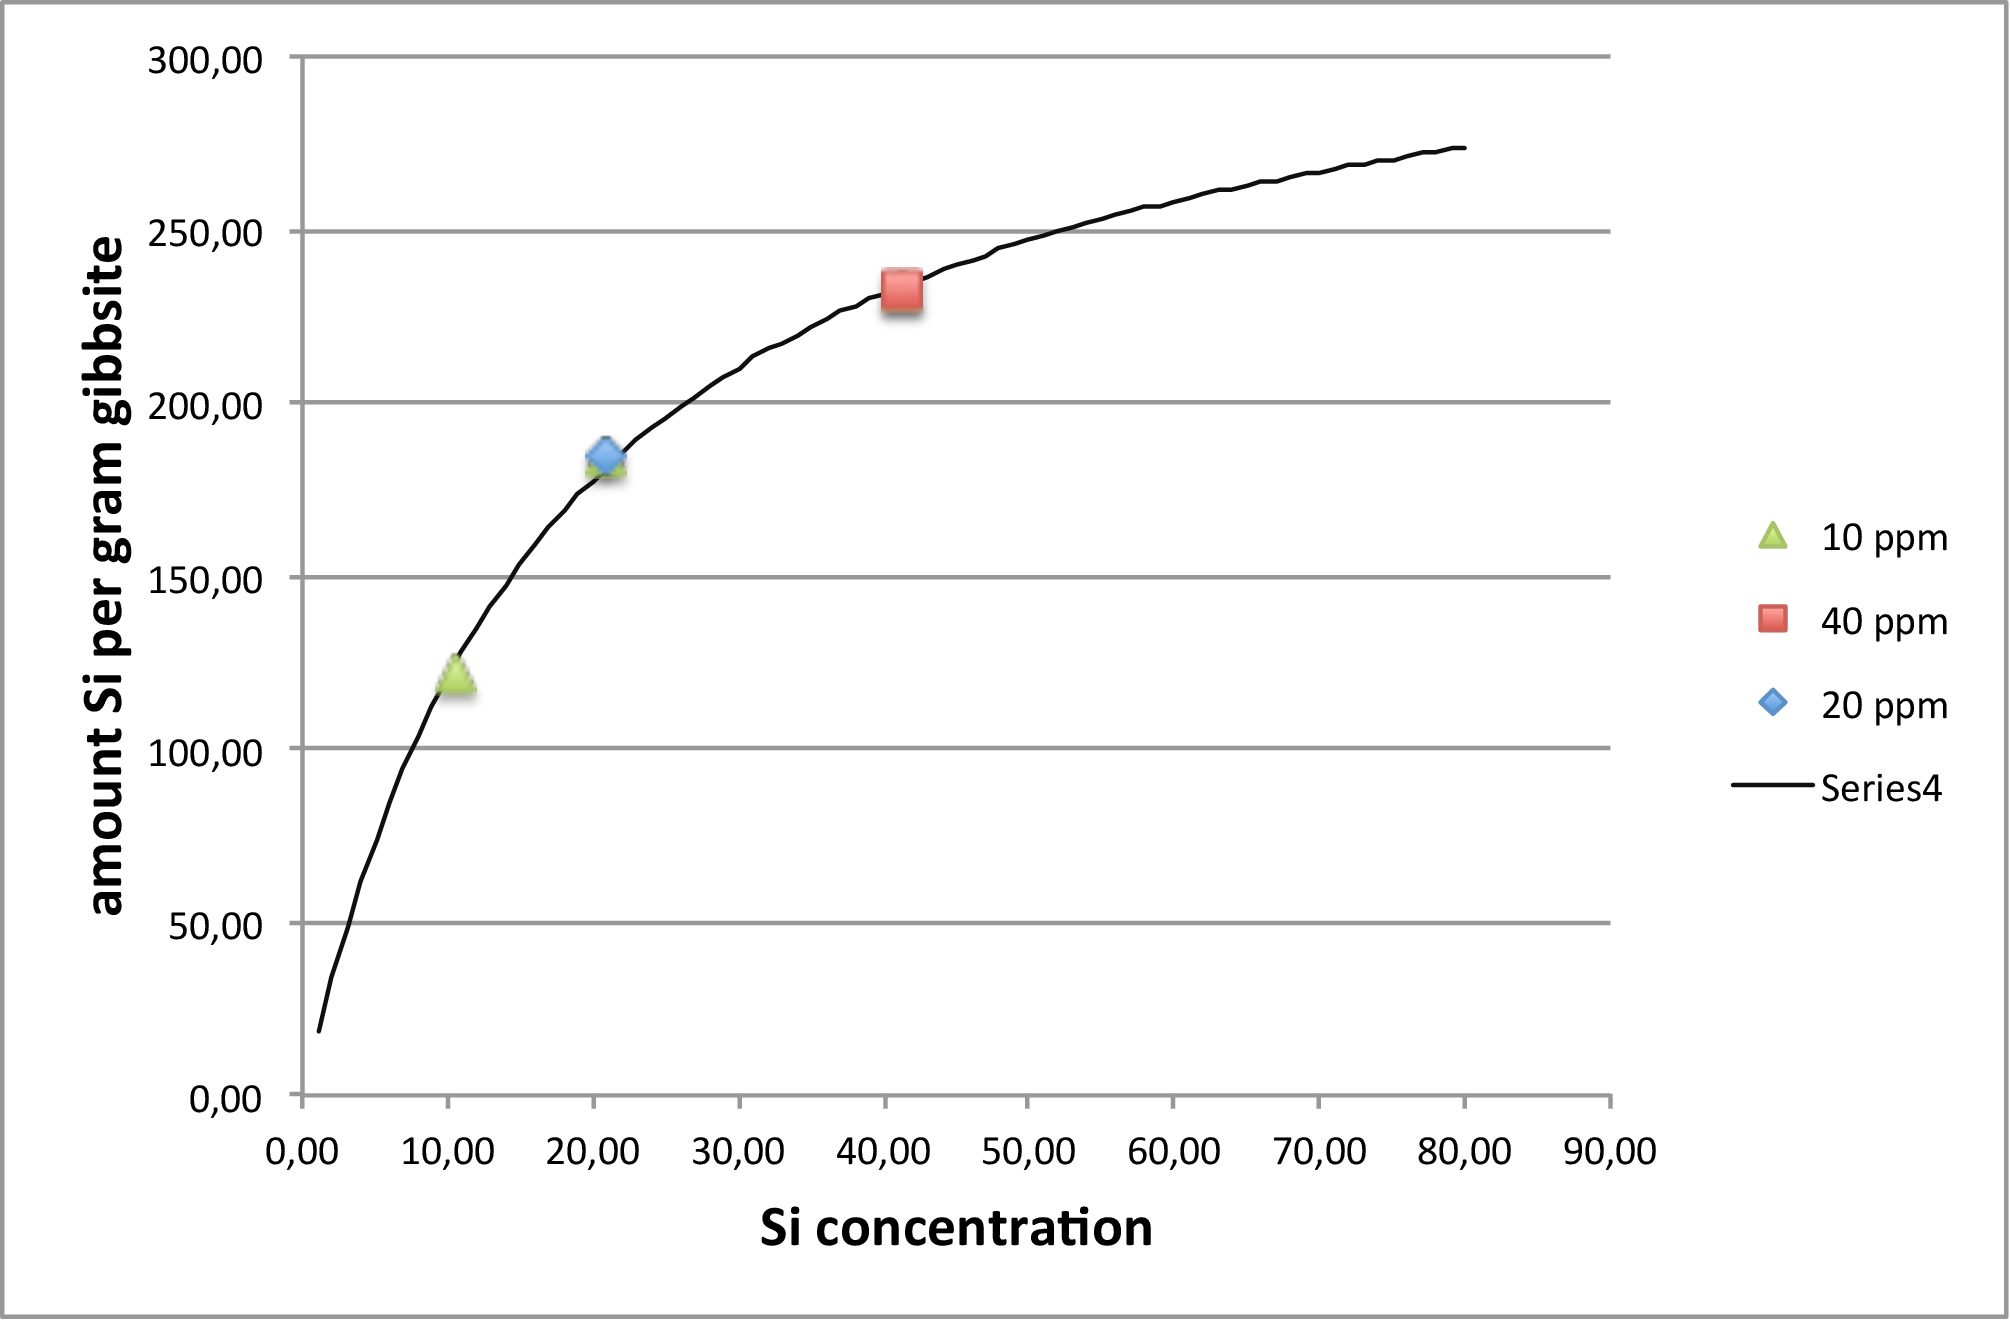
\includegraphics[width=0.7\columnwidth]{figures/langmuir_fig/langmuir_fig.png}
\caption{Menge Si adsorbiert pro Gramm Gibbsit gegen die initiale Si Konzentration. Schware Kurve Adsorptionsisotherme nach Langmuir (Gleichung 1)}
\end{center}
\end{figure}

Abbildung 1 zeigt die erreichte Beladung an Si pro Gramm Gibbsite gegen die initiale Si Konzentration der Experimente.


Lineraisieren nach Langmuir fuehrt zu Gleichung 2 und zur Abbildung 2:


\begin{equation}
\frac{[Si]}{q}=\frac{[Si]}{q_{max}}+\frac{1}{K*q{max}}
\end{equation}


\begin{figure}[h!]
\begin{center}
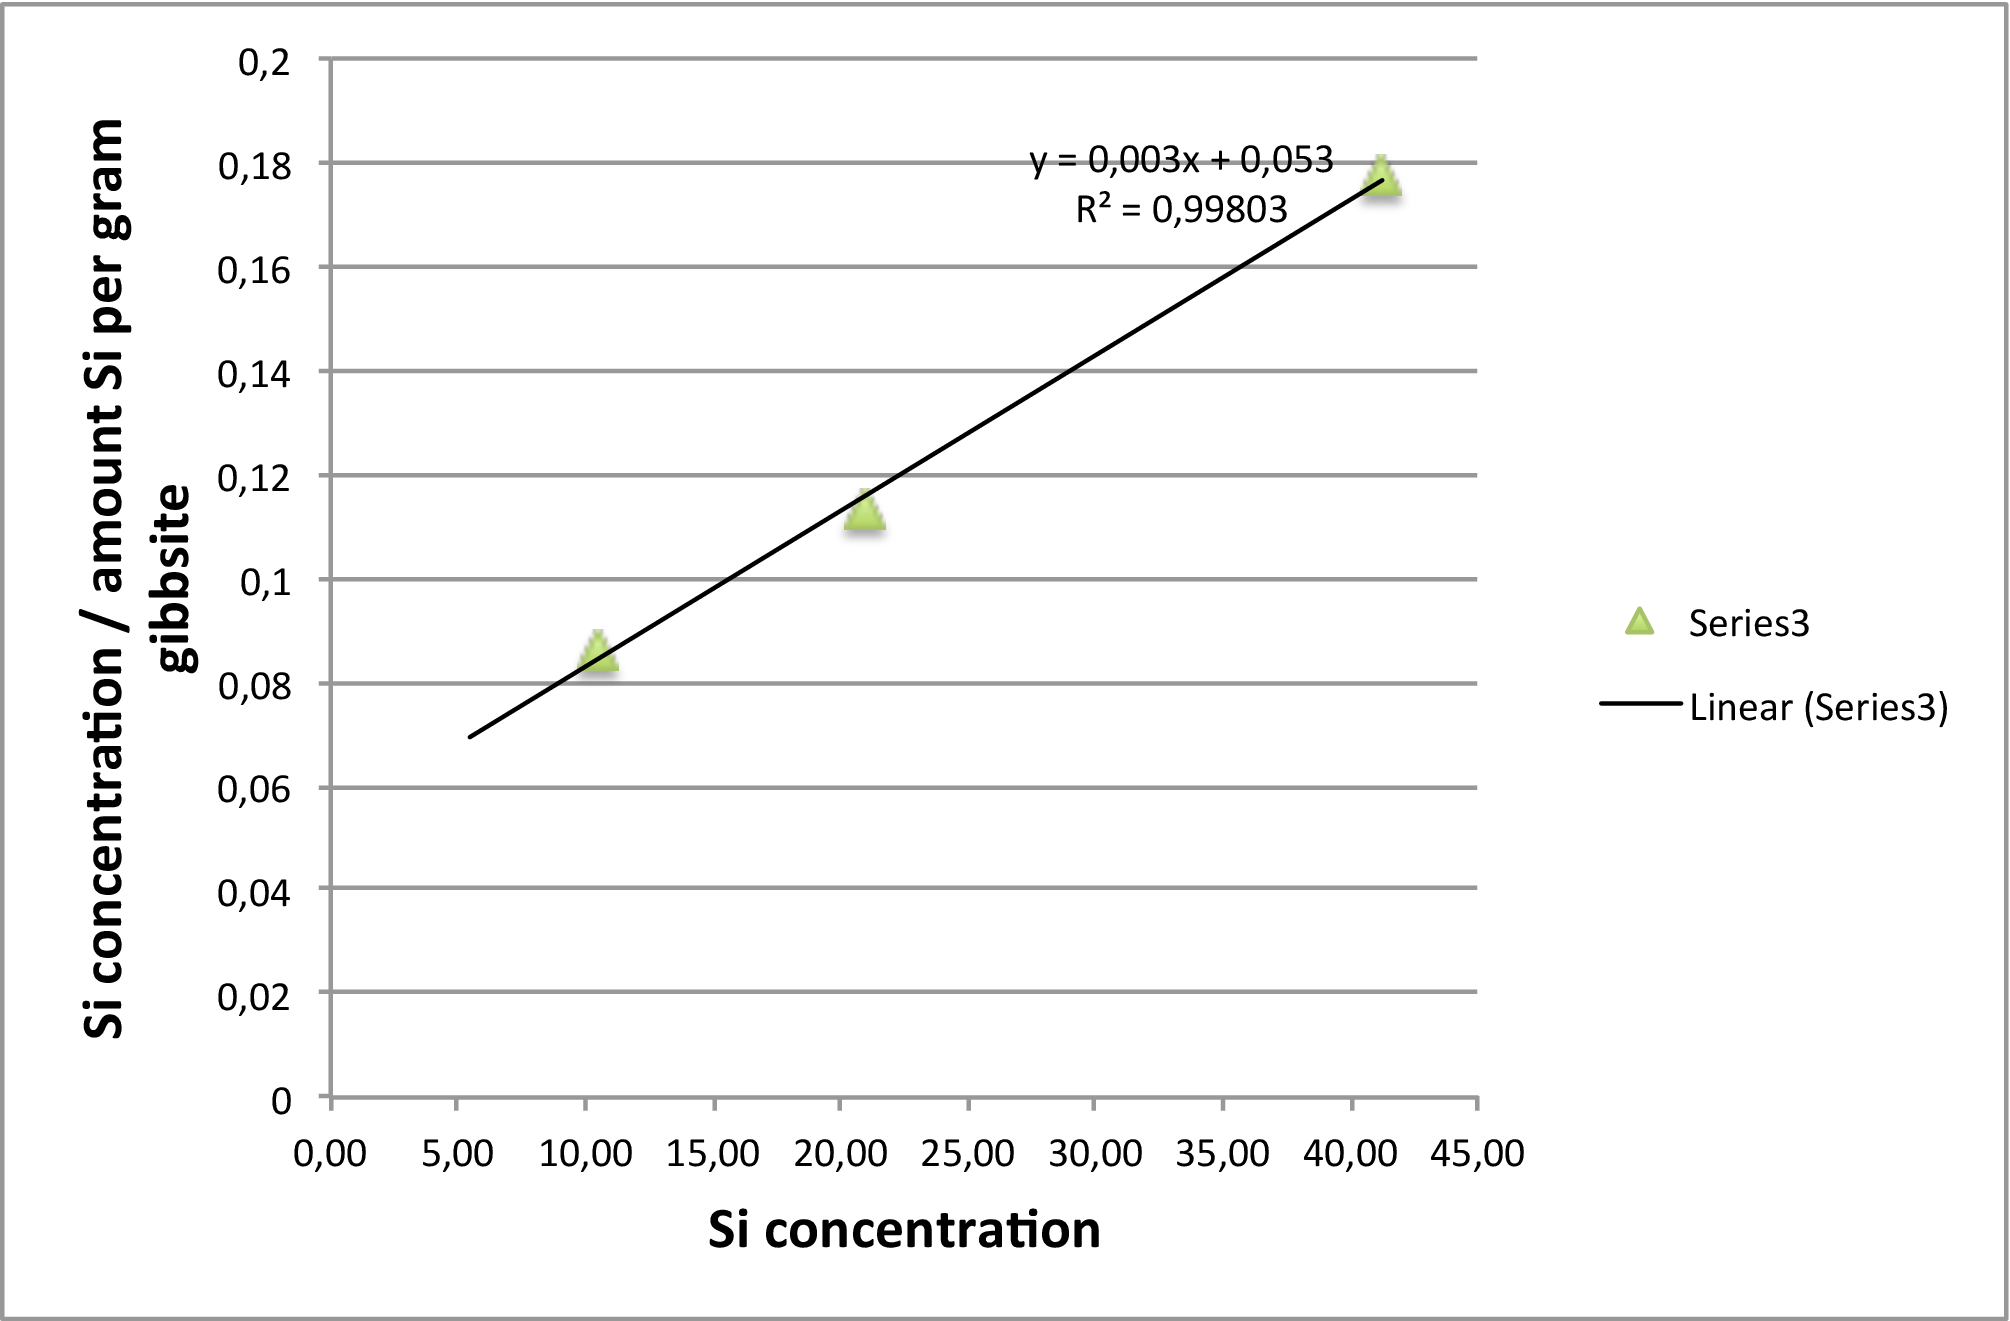
\includegraphics[width=0.7\columnwidth]{figures/langmuir_fig_lin/langmuir_fig_lin.png}
\caption{Si Konzentration geteilt durch die Menge Si adsorbiert pro Gramm Gibbsit ([Si]/q) gegen die Si Konzentration aufgetragen. Aus der Steigung kann man die maximale Beladung mit Si pro Gramm Gibbsite berechnen. }
\end{center}
\end{figure}

Aus der linearen Darstellung kann man aus der Steigung  eine maximale Beladung $q_{max}$ berechnen.
Dies ist hier $\sim$ 300$\mu$g Si pro Gramm Gibbsit ($1.2*10^{-5}$ mol Si pro Gramm Gibbsit)
Die maximal adsorbierte Menge in dieser Versuchsreihe waren  $\sim$ 230$\mu$g Si pro Gramm Gibbsite bei initial 40 ppm Si.


\end{document}

